\title{คาบเรียนที่ 12: การหาปริพันธ์โดยการแยกส่วน และการหาแทนค่าฟังก์ชันตรีโกณมิติ}
\frame{\titlepage}

\begin{frame}{สารบัญ}
\tableofcontents
\end{frame}

%%%%%%%%%%%%%%
\section[เทคนิคการแยกส่วน]{เทคนิคการหาปริพันธ์ - การแยกส่วน (by part)}
\frame{\sectionpage}
%%%%%%%%%%%%%%

\begin{frame}
ถ้ายังจำกันได้ เรามีสมบัติอนุพันธ์ของผลคูณ \pa
\[\dx (u\cdot v) = u \dx v + v \dx u \] \pa
ซึ่งเขียนในอีกรูปหนึ่งได้เป็น
\[ d (u \cdot v) = u \, dv + v \, du\] \pa
เราสามารถหาปริพันธ์ทั้งสองข้างได้เป็น
\begin{eqnarray*}
\int d(u\cdot v) &=& \int (u \, dv + v \, du) \\ \pa
&=& \left(\int u \,dv\right) + \left(\int v \,du\right) \pa
\end{eqnarray*}
ถ้าเรามอง $u \cdot v$ เป็นฟังก์ชันหนึ่ง \pa จะได้ $\displaystyle \int d(u\cdot v) \pa = \int 1 \, d(u \cdot v) \pa = u\cdot v + C$
\end{frame}

\begin{frame}
ฉะนั้น
\begin{eqnarray*}
uv + C &=& \left(\int u \, dv\right) + \left(\int v\, du\right) \\ \pa
\int u dv &=& uv + C - \left(\int v\, du\right) \pa
\end{eqnarray*}
แต่เนื่องจากค่า $C$ นี้จะไปรวมกับค่า $C$ จาก $\int v du$ อยู่แล้ว จึงไม่จำเป็นต้องเขียนตอนนี้ \pa
\begin{defn}{}{}
กำหนดให้ $u, v$ เป็นฟังก์ชันที่หาปริพันธ์ได้ แล้ว
\begin{eq} 
\int u \, dv = uv - \int v\, du
\end{eq}
\end{defn} 
\end{frame}

\begin{frame}
\begin{remark}{ขั้นตอนการหาปริพันธ์แยกส่วน}
\begin{enumerate}
\item สังเกตว่า $f$ จะเป็นฟังก์ชันหลายฟังก์ชันคูณกัน (หรือหารกัน)\pa แยกเป็นสองส่วนได้ $f = u\cdot v'$ โดยที่ $v'$ เป็นฟังก์ชันที่หาปริพันธ์ได้ง่าย \pa
\item เขียน $f \, dx = u \cdot v' \, dx = u \, dv$ \pa โดยที่ $v' \, dx = dv$ \pa นั่นคือ $v = \int v' \, dx$ โดยละพจน์ $C$ ไว้ \pa
\item แทนค่า $u$ และ $v$ ที่ได้ลงในสูตร 
\[ \int u \, dv = uv - \int v\, du\]
\end{enumerate}
\end{remark}
\end{frame}


\begin{frame}[t]
\begin{ex}
จงหาปริพันธ์ $\int x \sin x \, dx$
\end{ex} \pa
\begin{sol}
\begin{enumerate}
\item ให้ $f(x) = x \sin x$ \pa สังเกตว่าเป็นฟังก์ชันที่คูณกัน เราจึงให้ $u = x$ และ $v' = \sin x$ \pa
\item เมื่อ $v' = \sin x$ \pa จะได้ $v = \int \sin x \, dx = -\cos x + C$ \pa
\item แทนค่า $u = x$ และ $v = -\cos x$ ลงในสูตร \pa
\begin{eqnarray*}
\int u \, dv &=& uv - \int v\, du \\ \pa
\int x \sin x \, dx &=& (x) \cdot (-\cos x) - \int (-\cos x) \, dx \\ \pa
&=& -x\cos x + \sin x + C
\end{eqnarray*}
\end{enumerate}
\end{sol}
\end{frame}


\begin{frame}[t]
\begin{ex}
จงหาปริพันธ์ $\int x e^x \, dx$
\end{ex} \pa
\begin{sol}
\begin{enumerate}
\item ให้ $f(x) = x e^x$ \pa สังเกตว่าเป็นฟังก์ชันที่คูณกัน เราจึงให้ $u = x$ และ $v' = e^x$ \pa
\item เมื่อ $v' = e^x$ \pa จะได้ $v = \int e^x \, dx = e^x + C$ \pa
\item แทนค่า $u = x$ และ $v = e^x$ ลงในสูตร \pa
\begin{eqnarray*}
\int u \, dv &=& uv - \int v\, du \\ \pa
\int x e^x \, dx &=& (x) \cdot (e^x) - \int (e^x) \, d (x) \\ \pa
&=& xe^x - e^x + C
\end{eqnarray*}
\end{enumerate}
\end{sol}
\end{frame}


\begin{frame}[t]
\begin{ex}
จงหาปริพันธ์ $\int x^2 \ln x \, dx$
\end{ex}
\begin{sol}
\begin{enumerate}
\item ให้ $f(x) = x^2 \ln x$ \pa สังเกตว่าเป็นฟังก์ชันที่คูณกัน เราจึงให้ $u = x^2$ และ $v' = \ln x$ \pa
\item เมื่อ $v' = \ln x$ \pa จะได้ $v = \int \ln x \, dx = ........$ \pa
\item เนื่องจากเรายังไม่รู้ค่าของ $\int \ln x \, dx$ แปลว่าเราต้องลองเปลี่ยน $u, v'$ เป็นตัวอื่น \pa
\end{enumerate}
\end{sol}
\end{frame}


\begin{frame}[t]
\[\int x^2 \ln x \, dx\]
\begin{sol} (ต่อ)
\begin{enumerate}
\item ลองใหม่ ให้ $u = \ln x$ และ $v' = x^2$ \pa
\item เมื่อ $v' = x^2$ \pa จะได้ $v = \int x^2 \, dx = \frac{1}{3}x^3 + C$ \pa
\item แทนค่า $u = \ln x$ และ $v = \frac{1}{3}x^3$ ลงในสูตร \pa
\begin{eqnarray*}
\int u \, dv &=& uv - \int v\, du \\ \pa
\int x^2 \ln x \, dx &=& (\ln x) \cdot \left( \frac{1}{3}x^3\right) - \int \frac{1}{3}x^3\, d (\ln x)\\ \pa
\end{eqnarray*}
\end{enumerate}
\end{sol}
\end{frame}

\begin{frame}
\begin{sol} (ต่อ)
\begin{eqnarray*}
\int x^2 \ln x \, dx &=& (\ln x) \cdot \left( \frac{1}{3}x^3\right) - \int \frac{1}{3}x^3\, d (\ln x)\\ \pa
&=& \frac{1}{3} x^3 \ln x - \int \frac{1}{3}x^3 \cdot \frac{1}{x}\, dx\\ \pa
&=& \frac{1}{3} x^3 \ln x - \frac{1}{3} \int x^2\, dx\\ \pa
&=& \frac{1}{3} x^3 \ln x - \frac{1}{3}\left( \frac{1}{3}x^3 + C \right)\\ \pa
&=& \frac{1}{3} x^3 \ln x - \frac{1}{9}x^3 + C
\end{eqnarray*}
\end{sol}
\end{frame}


\begin{frame}[t]
\begin{ex}
จงหาปริพันธ์ $\int x^4 \ln x \, dx$
\end{ex} \pa
\begin{sol}
กำหนดให้ $u = \ln x$ และ $v' = x^4$ จะได้ 
\[v = \int x^4 \, dx = \frac{1}{5}x^5 + C\]
ฉะนั้นแทนค่า $u = \ln x$ และ $v = \frac{1}{5}x^5$ ลงในสูตรจะได้
\begin{eqnarray*}
\int x^4 \ln x \, dx &=& (\ln x) \cdot \left( \frac{1}{5}x^5\right) - \int \frac{1}{5}x^5\, d (\ln x)\\ \pa
&=& \frac{1}{5} x^5 \ln x - \frac{1}{5} \int x^5 \cdot \frac{1}{x}\, dx\\ \pa
&=& \frac{1}{5} x^5 \ln x - \frac{1}{5} \int x^4\, dx\pa = \frac{1}{5} x^5 \ln x - \frac{1}{25}x^5 + C
\end{eqnarray*}
\end{sol}
\end{frame}


\begin{frame}[t]
\begin{ex}
จงหาปริพันธ์ $\int x^2 e^x \, dx$
\end{ex}
\begin{sol}
\begin{enumerate}
\item ลองให้ $u = x^2$ และ $v' = e^x$ \pa
\item เมื่อ $v' = e^x$ \pa จะได้ $v = \int e^x \, dx = e^x + C$ \pa
\item แทนค่า $u = x^2$ และ $v = e^x$ ลงในสูตร จะได้\pa
\begin{eqnarray*}
\int x^2 e^x \, dx &=& (x^2) \cdot (e^x) - \int e^x \, d (x^2)\\ \pa
&=& x^2 e^x - \int e^x \cdot 2x \, dx  \pa = x^2 e^x - 2 \int xe^x \, dx
\end{eqnarray*}
\end{enumerate}
แต่! เราไม่มีสูตรของ $\int xe^x \, dx$\pa 
\end{sol}
\end{frame}

\begin{frame}
\begin{sol} (ต่อ)
อย่างไรก็ตามสังเกตว่าเลขชี้กำลังของ $x$ ลดลงจาก $x^2$ เหลือ $x^1 = x$\pa  

ฉะนั้น ถ้าเราใช้เทคนิคนี้อีกรอบน่าจะทำให้เลขชี้กำลังหายไป \pa

เราสามารถหา $\int xe^x \, dx$ ได้โดยแทนค่า $u = x$ และ $v = e^x$ ลงในสูตร \pa
\begin{eqnarray*}
\int u \, dv &=& uv - \int v\, du \\ \pa
\int x e^x \, dx &=& (x) \cdot (e^x) - \int (e^x) \, d (x) \\ \pa
&=& xe^x - e^x + C
\end{eqnarray*}
\end{sol}
\end{frame}

\begin{frame}
\begin{sol} (ต่อ)
ฉะนั้น เราแทนค่า $\int x e^x \, dx = xe^x - e^x + C$ ในสมการ จะได้
\begin{eqnarray*} 
\int x^2 e^x \pa &=& x^2 e^x - 2 \int xe^x \, dx \\ \pa
&=& x^2 e^x - 2 \left( xe^x - e^x + C \right) \\ \pa
&=& x^2 e^x - 2xe^x + 2e^x + C
\end{eqnarray*}
\end{sol}
\end{frame}


\begin{frame}[t]
\begin{ex}
จงหาปริพันธ์ $\int x^2 \sin x \, dx$
\end{ex}
\begin{sol}
\begin{enumerate}
\item ลองให้ $u = x^2$ และ $v' = \sin x$ \pa
\item เมื่อ $v' = \sin x$ \pa จะได้ $v = \int \sin x\, dx = -\cos x + C$ โดยละ $C$ ไว้เหลือ $v = -\cos x$ \pa
\item แทนค่า $u = x^2$ และ $v = -\cos x$ ลงในสูตร จะได้\pa
\begin{eqnarray*}
\int x^2 \sin x\, dx &=& (x^2) \cdot (-\cos x) - \int (-\cos x) \, d (x^2)\\ \pa
&=& -x^2 \cos x + \int \cos x \cdot 2x \, dx \\ \pa
&=& -x^2 \cos x+ 2 \int x \cos x\, dx
\end{eqnarray*}
\end{enumerate}
สังเกตว่า แม้จะหาปริพันธ์ไม่ได้ในทันที แต่เลขชี้กำลังก็ลดลงมาจาก $x^2$ เหลือ $x$
\end{sol}
\end{frame}

\begin{frame}
\begin{sol} (ต่อ)
ใช้เทคนิคปริพันธ์แยกส่วนอีกรอบ กับ $\int x \cos x \, dx$ โดยแทน $u = x$ และ $dv = \cos x \, dx$ นั่นคือ $v = \sin x$ ลงไปในสูตร \pa
\begin{eqnarray*}
\int u \, dv &=& uv - \int v\, du \\ \pa
\int x \cos x\, dx &=& (x) \cdot (\sin x) - \int (\sin x) \, d (x) \\ \pa
&=& x\sin x + \cos x + C
\end{eqnarray*}
\end{sol}
\end{frame}

\begin{frame}
\begin{sol} (ต่อ)
ฉะนั้น เราแทนค่า $\int x \cos x \, dx = x\sin x + \cos x + C$ ในสมการ จะได้
\begin{eqnarray*} 
\int x^2 \sin x \pa &=& -x^2 \cos x + 2 \int x \cos x \, dx \\ \pa
&=& -x^2 \cos x + 2(x\sin x + \cos x + C)\\ \pa
&=& -x^2 \cos x + 2x\sin x + 2\cos x + C
\end{eqnarray*}
\end{sol}
\end{frame}


%%%%%%%%%%%%%%
\section[แทนค่าด้วยฟังก์ชันตรีโกณฯ]{การหาปริพันธ์โดยการแทนค่าด้วยฟังก์ชันตรีโกณมิติ}
\frame{\sectionpage}
%%%%%%%%%%%%%%

\begin{frame}
เราทราบว่าเราสามารถหาปริพันธ์
\[ \int \sin^{10} x \cos x \, dx\]
ได้ ด้วยการแทนค่า $u = \sin x$ จะได้เป็น
\[ \int u^{10} \, du\]
ต่อไปนี้ เราจะแทนค่าด้วยฟังก์ชันตรีโกณมิติ แต่จะอยู่ในรูปแบบ
\[ x = \frac{a}{b} \sin \theta, \quad \frac{a}{b} \tan \theta, \quad \frac{a}{b} \sec \theta\]
สังเกตว่า รูปแบบจะต่างจากเดิม คือแทนที่จะสร้างตัวแปรใหม่ $u$ ให้เป็น $\sin x$ ที่เป็นตัวแปรเดิม แต่เป็นการให้ตัวแปรเดิม $x$ เป็น $\sin \theta$ ของตัวแปรใหม่แทน
\end{frame}

\begin{frame}[t]
\frametitle{ที่มา}
กำหนดพจน์
\[ \sqrt{1-\sin^2 x}\]
\begin{slide}
เราสามารถใช้เอกลักษณ์ตรีโกณมิติที่ว่า $\sin^2 x+ \cos^2 x = 1$ มาจัดรูปใหม่ได้เป็น
\[ \sqrt{1-\sin^2 x} = \sqrt{\cos^2 x} = \pm \cos x\]
ในทำนองเดียวกัน ถ้ามีพจน์
\[ \sqrt{4 - x^2}\]
เราสามารถกำหนดตัวแปรใหม่ โดยให้ $x = 2\sin \theta$ เพื่อให้ได้
\[ \sqrt{4 - x^2} = \sqrt{4 - (2\sin \theta)^2} = \sqrt{4 - 4\sin^2 \theta} = 2\sqrt{1-\sin^2 \theta} = \pm 2 \cos \theta\]
ทำให้สามารถขจัดพจน์รากได้
\end{slide}
\end{frame}

\begin{frame}[t]
ในทำนองเดียวกัน เรามีเอกลักษณ์ตรีโกณมิติดังนี้
\begin{remark}{}
\[\sqrt{1-\sin^2 x} = \pm \cos x, \sqrt{1 + \tan^2 x} = \pm \sec x, \sqrt{\sec^2 - 1} = \pm \csc x\]
\end{remark}
\begin{sol}
เราได้พิสูจน์ข้อ 1 ไปแล้ว เราจะพิสูจน์ข้อ 2 และทิ้งข้อ 3 ไว้เป็นแบบฝึกหัด
\begin{eq*}
\sqrt{1 + \tan^2 x} = \sqrt{1 + \frac{\sin^2 x}{\cos^2 x}} &=& \sqrt{\frac{\cos^2 x}{\cos^2 x} + \frac{\sin^2 x}{\cos^2 x}} \\
&=& \sqrt{\frac{1}{\cos^2 x}} \\
&=& \pm \frac{1}{\cos x} = \pm \sec x
\end{eq*}
\end{sol}
\end{frame}

\begin{frame}
\begin{remark}{}
\begin{enumerate}
\item ถ้าปริพันธ์อยู่ในรูป $\sqrt{a^2 - b^2 x^2}$ หรือ $a^2 - b^2 x^2$ ให้แทนค่า
\[ x = \frac{a}{b} \sin \theta\]
\item ถ้าปริพันธ์อยู่ในรูป $\sqrt{a^2 + b^2 x^2}$ หรือ $a^2 + b^2 x^2$ ให้แทนค่า
\[ x = \frac{a}{b} \tan \theta\]
\item ถ้าปริพันธ์อยู่ในรูป $\sqrt{b^2 x^2 - a^2 }$ หรือ $ b^2 x^2 -  a$ ให้แทนค่า
\[ x = \frac{a}{b} \sin \theta\]
\end{enumerate}
\end{remark}
เมื่อแทนค่าแล้ว ให้ทำการเปลี่ยน $dx$ เป็น $d\theta$ และจัดรูปจนเหลือแต่ตัวแปร $\theta$ และใช้เทคนิคการหาปริพันธ์จนได้คำตอบ
\end{frame}

\begin{frame}{การแปลงฟังก์ชันตรีโกณมิติ เมื่อกำหนดให้ $x = \frac{a}{b} \sin \theta$}
\begin{columns}
\begin{column}{0.4\textwidth}
จาก $x = \frac{a}{b} \sin \theta$ จะได้
\[\sin \theta = \frac{bx}{a}\]
เมื่อสร้างสามเหลี่ยมมุมฉากที่มีมุม $\theta$ แล้วจะได้ว่า
\begin{eq*} 
\cos \theta &=& \frac{\sqrt{a^2-bx^2}}{a} \\
\tan \theta &=& \frac{bx}{\sqrt{a^2-bx^2}}
\end{eq*}
เป็นต้น
\end{column}
\begin{column}{0.4\textwidth}
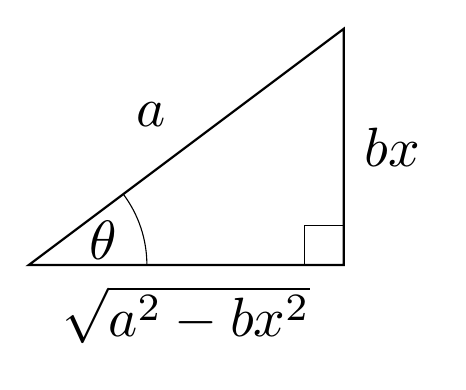
\begin{tikzpicture}[every node/.style = {scale = 2}]
\draw[thick] (0,0) -- node[pos = 0.5, below] {$\sqrt{a^2-bx^2}$} (4,0) -- node[pos = 0.5, right] {$bx$} (4,3) -- node[pos = 0.5, above left] {$a$} cycle;
\draw (1.5,0) arc [start angle = 0, end angle = 37, radius = 1.5] ;
\draw (4,0) rectangle (3.5, 0.5);
\node at (18.5: 1) {$\theta$};
\end{tikzpicture}
\end{column}
\end{columns}
\end{frame}

\begin{frame}{การแปลงฟังก์ชันตรีโกรณมิติ เมื่อกำหนดให้ $x = \frac{a}{b} \tan \theta$}
\begin{columns}
\begin{column}{0.4\textwidth}
จาก $x = \frac{a}{b} \tan \theta$ จะได้
\[\tan \theta = \frac{bx}{a}\]
เมื่อสร้างสามเหลี่ยมมุมฉากที่มีมุม $\theta$ แล้วจะได้ว่า
\begin{eq*} 
\sin \theta &=& \frac{bx}{a^2 + b^2x^2} \\
\cos \theta &=& \frac{a}{a^2 + b^2x^2}
\end{eq*}
เป็นต้น
\end{column}
\begin{column}{0.4\textwidth}
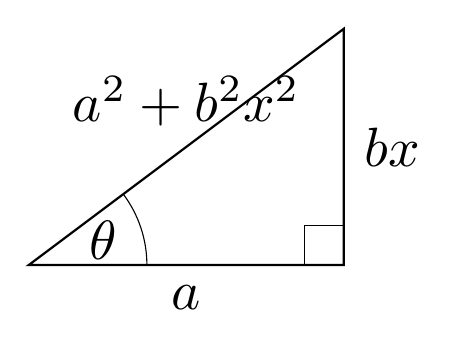
\begin{tikzpicture}[every node/.style = {scale = 2}]
\draw[thick] (0,0) -- node[pos = 0.5, below] {$a$} (4,0) -- node[pos = 0.5, right] {$bx$} (4,3) -- node[pos = 0.5, above ] {$a^2 + b^2x^2$} cycle;
\draw (1.5,0) arc [start angle = 0, end angle = 37, radius = 1.5] ;
\draw (4,0) rectangle (3.5, 0.5);
\node at (18.5: 1) {$\theta$};
\end{tikzpicture}
\end{column}
\end{columns}
\end{frame}



\begin{frame}[t]
\begin{ex}
จงหาปริพันธ์ $\int \sqrt{1 - x^2} \, dx$
\end{ex} \pa
\begin{sol}
เนื่องจากพจน์ $1 - x^2$ อยู่ในรูปแบบที่ 1 โดยถ้าเทียบ $1 - x^2 = a^2 - b^2 x^2$ จะได้ $a=1$ และ $b=1$ ดังนั้นจึงกำหนดให้
\[ x = \sin \theta \qquad \rightarrow \qquad dx = \cos \theta \, d\theta\]
ฉะนั้น
\begin{eqnarray*}
\int \sqrt{1-x^2} \, dx &=& \int \sqrt{1 - \sin^2 \theta} (\cos \theta \, d\theta) \\
&=& \int (\cos \theta) (\cos \theta) \, d\theta \\
&=& \int \cos^2 \theta \, d\theta \\
\end{eqnarray*}
\end{sol}
\end{frame}

\begin{frame}[t]
\begin{sol} (ต่อ)
จากนั้น ใช้เอกลักษณ์ตรีโกณมิติ $\cos^2 \theta = \frac{\cos (2\theta) + 1}{2}$ จะได้
\begin{eq*}
\int \cos^2 \theta \, d\theta &=& \frac{1}{4}\sin (2\theta) - \frac{1}{2}\theta + C \\
&=& \frac{1}{2} \sin \theta \cos \theta + \frac{1}{2} \theta + C \\
\end{eq*}
สุดท้าย แปลงกลับเป็นตัวแปร $x$ ได้
\[ \sin \theta = x \qquad \cos \theta = \sqrt{1-x^2} \qquad \theta = \arcsin x\]
นั่นคือ
\[\frac{1}{2} \sin \theta \cos \theta + \frac{1}{2} \theta + C = \frac{1}{2} x\sqrt{1-x^2} + \frac{1}{2} \arcsin x + C \]
\end{sol}
\end{frame}


\begin{frame}[t]
\begin{ex}
จงหาปริพันธ์ $\int (1 - x^2)^{\frac{3}{2}} \, dx$
\end{ex} \pa
\begin{sol}
เนื่องจากพจน์ $1 - x^2$ อยู่ในรูปแบบที่ 1 โดยถ้าเทียบ $1 - x^2 = a^2 - b^2 x^2$ จะได้ $a=1$ และ $b=1$ ดังนั้นจึงกำหนดให้
\[ x = \sin \theta\]
เมื่อแทนค่าจะได้
\begin{eqnarray*}
(1 - x^2)^{\frac{3}{2}} &=& \left( 1 - \sin^2 \theta \right)^{\frac{3}{2}} \\
&=& \left( \cos^2 \theta \right)^{\frac{3}{2}} \\
&=& \cos^3 \theta
\end{eqnarray*}
\end{sol}
\end{frame}

\begin{frame}[t]
\begin{sol} (ต่อ)
นอกจากนี้ จาก $x = \sin \theta$ จะได้ $dx = \cos \theta \, d\theta$ ฉะนั้น เมื่อเราเปลี่ยนตัวแปร $x$ ทั้งหมดให้เป็น $\theta$ จะได้
\begin{eq*}
\int (1 - x^2)^{\frac{3}{2}} \, dx &=& \int  \cos^3 \theta \left( \cos \theta \, d\theta\right) \\
&=& \int \cos^4 \theta \, d\theta
\end{eq*}
ซึ่งกลายเป็นปริพันธ์ในรูปแบบของฟังก์ชันตรีโกณมิติชี้กำลัง ที่เราได้เคยศึกษาไว้แล้ว ในที่นี้เราจะใช้เอกลักษณ์
\[\cos^4 \theta = \frac{1}{8} \cos (4\theta) - \frac{1}{2}\cos (2\theta) + \frac{3}{8}\]
เมื่อทำการหาปริพันธ์แต่ละพจน์แยกกัน จะได้
\[ \int \cos^4 \theta \, d\theta = \frac{1}{32} \sin (4\theta) - \frac{1}{4} \sin (2\theta) + \frac{3}{8}\theta + C\]
\end{sol}
\end{frame}

\begin{frame}[t]
\begin{sol} (ต่อ) ดังนั้น
\begin{eq*}
\int (1 - x^2)^{\frac{3}{2}} \, dx &=&  \frac{1}{32} \sin (4\theta) - \frac{1}{4} \sin (2\theta) + \frac{3}{8}\theta + C
\end{eq*}
สุดท้าย การจะเปลี่ยน $\theta$ ให้กลับไปเป็น $x$ ต้องใช้การแทนค่า $x = \sin \theta$ และสมบัติว่า $\cos \theta = \sqrt{1 - \sin^2\theta} = \sqrt{1-x^2}$ ได้ดังนี้
\begin{eq*}
\theta &=& \arcsin x \\
\sin (2\theta) &=& 2 \sin \theta \cos \theta \\
&=& 2 x \sqrt{1-x^2} \\
\sin (4 \theta) &=& 2 \sin (2 \theta) \cos (2\theta) = 2 \sin (2\theta) (2\sin^2 \theta - 1) \\
&=& 2 x \sqrt{1-x^2} (2x^2-1)
\end{eq*}
ฉะนั้น
\[\int (1 - x^2)^{\frac{3}{2}} \, dx = \frac{1}{32} 2 x \sqrt{1-x^2} (2x^2-1) - \frac{1}{4} 2 x \sqrt{1-x^2} + \frac{3}{8} \arcsin x + C\]
\end{sol}
\end{frame}


\begin{frame}[t]
\begin{ex}
จงหาปริพันธ์ $\int \frac{1}{x \sqrt{9+4x^2}} \, dx$
\end{ex}
\begin{sol}
เนื่องจากพจน์ $9 + 4x^2$ อยู่ในรูปแบบที่ 2 โดยถ้าเทียบ $9 + 4x^2 = a^2 + b^2 x^2$ จะได้ $a=3$ และ $b=2$ ดังนั้นจึงกำหนดให้
\[ x = \frac{3}{2} \tan \theta\]
เมื่อแทนค่าจะได้
\begin{eqnarray*}
\sqrt{9 + 4x^2} = \sqrt{ 9 + 4\left(\frac{4}{3} \tan \theta\right)^2 } &=& \sqrt{9 +  9 \tan^2 \theta} \\
&=& \sqrt{9} \sqrt{1 + \tan^2 \theta} \\
&=& 3 \sec \theta
\end{eqnarray*}
\end{sol}
\end{frame}

\begin{frame}[t]
\begin{sol} (ต่อ)
นอกจากนี้ จาก $x = \frac{3}{2} \tan \theta$ จะได้ $dx = \frac{3}{2} \sec^2 \theta \, d\theta$ ฉะนั้น เมื่อเราเปลี่ยนตัวแปร $x$ ทั้งหมดให้เป็น $\theta$ จะได้
\begin{eq*}
\int \frac{1}{x \sqrt{9+4x^2}} \, dx &=& \int \frac{1}{\left( \frac{3}{2} \tan \theta\right) (3 \sec \theta)} \left( \frac{3}{2} \sec^2 \theta \, d\theta\right) \\
&=&\frac{1}{3} \int \frac{\sec \theta}{\tan \theta} \, d\theta \\
&=& \frac{1}{3} \int \csc \theta \, d\theta \\
&=& \frac{1}{3} \ln | \csc \theta - \cot \theta | + C \mathnote{สูตรปริพันธ์ $\csc \theta$}\\
\end{eq*}

\end{sol}
\end{frame}

\begin{frame}[t]
\begin{sol} (ต่อ)
สุดท้าย การจะเปลี่ยน $\theta$ กลับไปเป็น $x$ ต้องอาศัยการวาดสามเหลี่ยมมุมฉากที่มีมุม $\theta$ ซึ่ง $x = \frac{3}{2} \tan \theta$ นั่นคือ $\tan \theta = \frac{2x}{3}$ ทำให้ด้านประกอบมุมฉากยาว $2x$ และ $3$ ตามลำดับ ด้านตรงข้ามมุมฉากจึงมีความยาวเท่ากับ $\sqrt{(2x)^2 + 3^2} = \sqrt{4x^2+9}$

\begin{columns}
\begin{column}{0.4\textwidth}
จากภาพ จะได้
\begin{eq*} 
\csc \theta &=& \frac{1}{\sin \theta} = \frac{\sqrt{4x^2+9}}{2x} \\
\cot \theta &=& \frac{3}{2x}
\end{eq*}
ฉะนั้น คำตอบคือ
\end{column}
\begin{column}{0.4\textwidth}
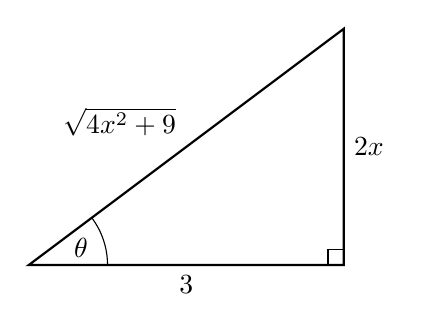
\begin{tikzpicture}
\draw[thick] (0,0) -- node[pos = 0.5, below] {3} (4,0) -- node[pos = 0.5, right] {$2x$} (4,3) -- node[pos = 0.5, above left] {$\sqrt{4x^2+9}$} cycle;
\draw (1,0) arc [start angle = 0, end angle = 37, radius = 1] ;
\draw (4,0) rectangle (3.8, 0.2);
\node at (18.5: 0.7) {$\theta$};
\end{tikzpicture}
\end{column}
\end{columns}

\[\frac{1}{3} \ln | \csc \theta - \cot \theta | + C = \frac{1}{3} \ln \left| \frac{\sqrt{4x^2+9}}{2x} - \frac{3}{2x}\right| + C \]
\end{sol}
\end{frame}
